\documentclass[tikz]{standalone}
% \usepackage{amsmath}
\usetikzlibrary{arrows,decorations.markings,fit,matrix,positioning,shapes}
\tikzset{
    % >=latex,
    mymatrix/.style={matrix of nodes, nodes=typetag, row sep=.2em},
    mycontainer/.style={draw=gray, inner sep=.1ex},
    typetag/.style={draw=gray, inner sep=1ex, anchor=west},
    title/.style={draw=none, color=gray, inner sep=0pt},
    arrowfwd/.style={decoration={markings,mark=at position 1 with {\arrow[scale=2,>=stealth]{>}}},postaction={decorate}},
    arrowboth/.style={decoration={markings,mark=at position 0.15 with {\arrow[scale=2,>=stealth]{<}},mark=at position 1 with {\arrow[scale=2,>=stealth]{>}}},postaction={decorate}},
    borderthick/.style={draw,draw=black!50,thick},
    recwht/.style={draw,minimum width=3cm,minimum height=2cm,align=center,text width=3cm,text=black,fill=white,draw=black!50,thick},
    recred/.style={draw,minimum width=3cm,minimum height=2cm,align=center,text width=3cm,text=black,fill=red!30,draw=black!50,thick},
    squorg/.style={draw,minimum width=2cm,minimum height=2cm,align=center,text width=2cm,text=orange,fill=white,draw=orange!50,thick},
    rndred/.style={rounded corners=1cm,draw,minimum width=3cm,minimum height=2cm,align=center,text width=3cm,text=red,fill=rwhite,draw=red!30,thick},
    rndyel/.style={rounded corners=1cm,draw,minimum width=3cm,minimum height=2cm,align=center,text width=3cm,text=yellow,fill=white,draw=yellow!50,thick},
    diared/.style={diamond,draw,minimum width=3cm,minimum height=2cm,align=center,text width=3cm,text=red,fill=white,draw=red!30,thick,aspect=1.5},
    diayel/.style={diamond,draw,minimum width=3cm,minimum height=2cm,align=center,text width=3cm,text=yellow,fill=white,draw=yellow!50,thick,aspect=1.5},
    cirblu/.style={circle,draw,minimum width=2cm,minimum height=2cm,align=center,text width=2cm,text=blue,fill=white,draw=blue!50,very thick},
    cirred/.style={circle,draw,minimum width=2cm,minimum height=2cm,align=center,text width=2cm,text={rgb:red,255;green,0;blue,122},fill=white,draw={rgb:red,255;green,0;blue,122},very thick},
    cirpur/.style={circle,draw,minimum width=2cm,minimum height=2cm,align=center,text width=2cm,text={rgb:red,130;green,60;blue,250},fill=white,draw={rgb:red,130;green,60;blue,250},very thick},
    cylwht/.style={cylinder,draw,shape aspect=.5,cylinder uses custom fill,cylinder end fill=white,minimum width=1cm,minimum height=1cm,cylinder body fill=white,opacity=1,scale=2,draw=black!50,thick,rotate=90}
}
\begin{document}
    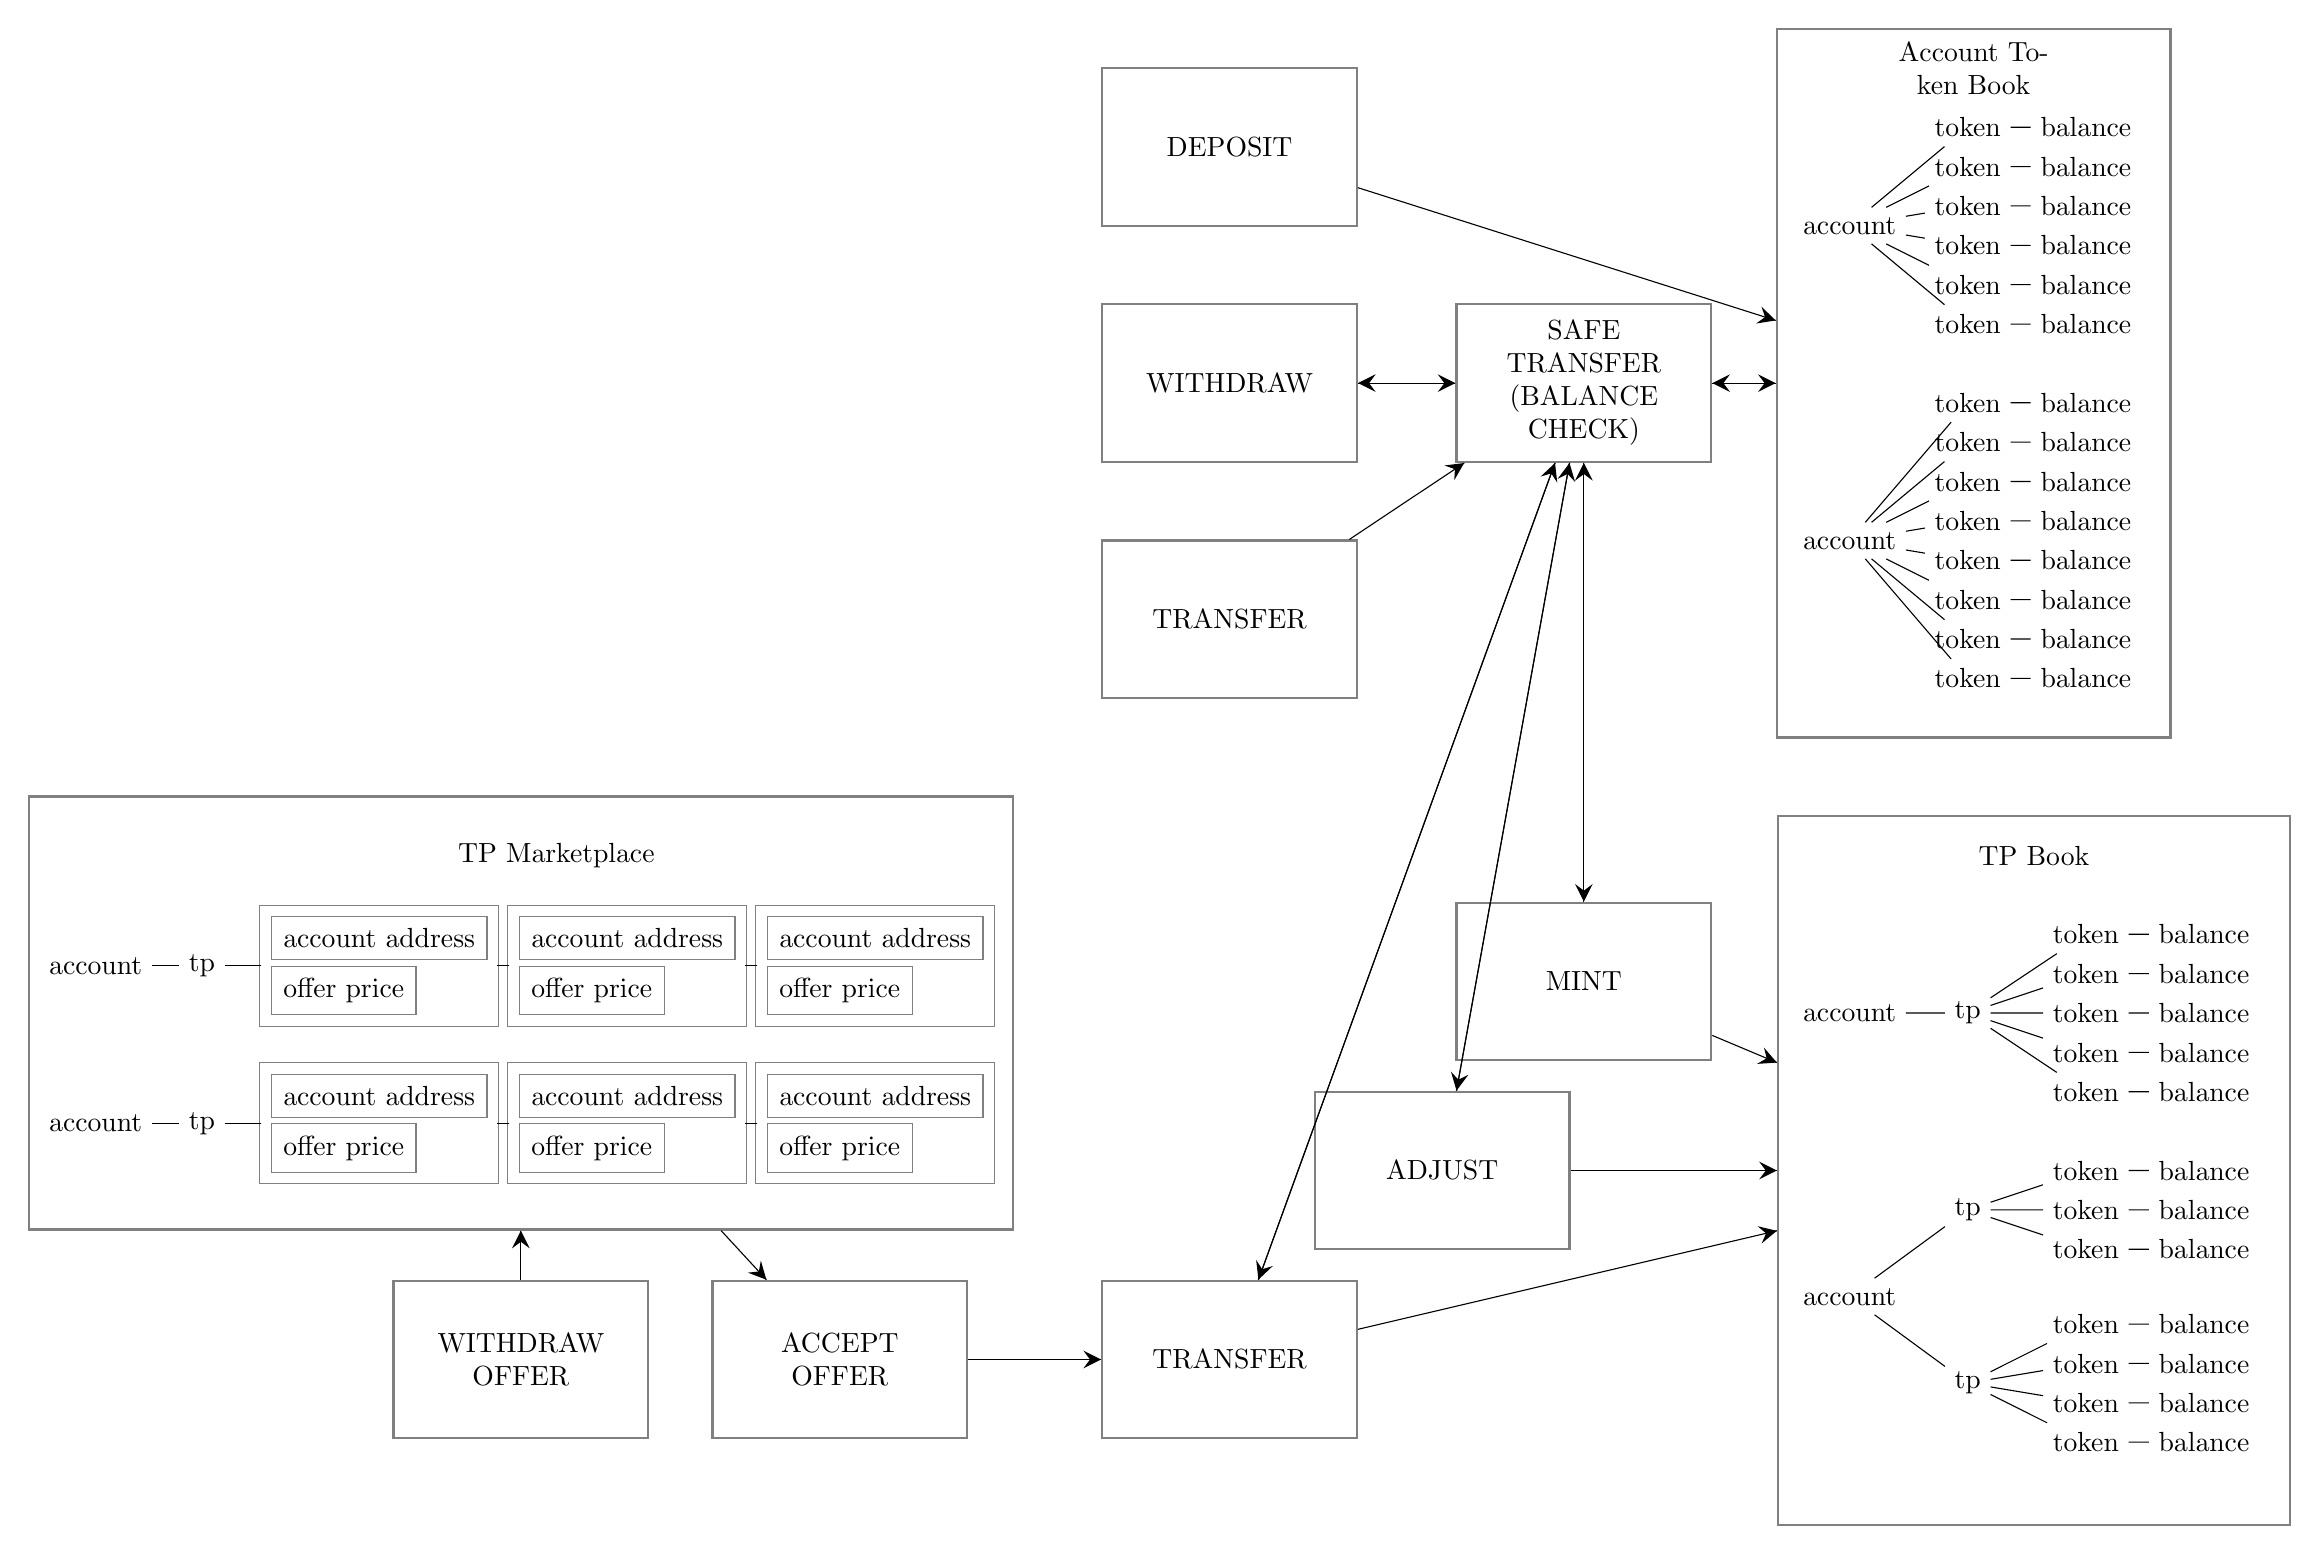
\begin{tikzpicture}[x=4.5cm,y=2cm]
        % Balance Book tree
        \node[style={draw,minimum width=5cm,minimum height=9cm,draw=black!50,thick}] (bbtreeoutline) at (0,0) {};
        \node[style={align=center,text width=3cm,text=black}] (bbtitle) at (0,2) {Account Token Book};
        \node (bbtree1) at (-.35,1) {account}[
                grow=east,
                level 1/.style = {sibling distance=.5cm}
            ]
            child {node {token} child {node {balance}} }
            child {node {token} child {node {balance}} }
            child {node {token} child {node {balance}} }
            child {node {token} child {node {balance}} }
            child {node {token} child {node {balance}} }
            child {node {token} child {node {balance}} };
        \node (bbtree2) at (-.35,-1) {account}[
                grow=east,
                level 1/.style = {sibling distance=.5cm}
            ]
            child {node {token} child {node {balance}} }
            child {node {token} child {node {balance}} }
            child {node {token} child {node {balance}} }
            child {node {token} child {node {balance}} }
            child {node {token} child {node {balance}} }
            child {node {token} child {node {balance}} }
            child {node {token} child {node {balance}} }
            child {node {token} child {node {balance}} };
        % Balance Book Actions
        \node[recwht] (bbdeposit1) at (-2.1,1.5) {DEPOSIT};
        \node[recwht] (bbwithdraw1) at (-2.1,0) {WITHDRAW};
        \node[recwht] (bbtransfer1) at (-2.1,-1.5) {TRANSFER};
        \node[recwht] (bbsafetransfer1) at (-1.1,0) {SAFE TRANSFER\\(BALANCE\\CHECK)};

        % TP Book tree
        \node[style={draw,minimum width=6.5cm,minimum height=9cm,draw=black!50,thick}] (tptreeoutline) at (.17,-5) {};
        \node[style={align=center,text width=3cm,text=black}] (tptitle) at (.17,-3) {TP Book};
        \node (tptree1) at (-.35,-4) {account}[
                grow=east,
                level 1/.style = {sibling distance=2.2cm},
                level 2/.style = {sibling distance=.5cm}
            ]
            child {node {tp}
                child {node {token} child {node {balance}} }
                child {node {token} child {node {balance}} }
                child {node {token} child {node {balance}} }
                child {node {token} child {node {balance}} }
                child {node {token} child {node {balance}} }
            };
        \node (tptree2) at (-.35,-5.8) {account}[
                grow=east,
                level 1/.style = {sibling distance=2.2cm},
                level 2/.style = {sibling distance=.5cm}
            ]
            child {node {tp}
                child {node {token} child {node {balance}} }
                child {node {token} child {node {balance}} }
                child {node {token} child {node {balance}} }
                child {node {token} child {node {balance}} }
            }
            child {node {tp}
                child {node {token} child {node {balance}} }
                child {node {token} child {node {balance}} }
                child {node {token} child {node {balance}} }
            };
        % TP Actions
        \node[recwht] (tpmint1) at (-1.1,-3.8) {MINT};
        \node[recwht] (tpadjust1) at (-1.5,-5) {ADJUST};
        \node[recwht] (tptransfer1) at (-2.1,-6.2) {TRANSFER};

        % TP Marketplace
        \node[style={draw,minimum width=12.5cm,minimum height=5.5cm,draw=black!50,thick}] (tpmktoutline) at (-4.1,-4) {};
        \node[style={align=center,text width=3cm,text=black}] (tpmkttitle) at (-4,-3) {TP Marketplace};
        \node (tpmkt1account) at (-5.3,-3.7) {account};
        \node (tpmkt1tp) at (-5,-3.7) {tp};
        \matrix[mymatrix] (tpmkt1o1) at (-4.5,-3.7) {
            % |[title]|OfferDetail \\
            account address \\
            offer price \\
        };
        \node[mycontainer, fit=(tpmkt1o1)] {};
        \matrix[mymatrix] (tpmkt1o2) at (-3.8,-3.7) {
            account address \\
            offer price \\
        };
        \node[mycontainer, fit=(tpmkt1o2)] {};
        \matrix[mymatrix] (tpmkt1o3) at (-3.1,-3.7) {
            account address \\
            offer price \\
        };
        \node[mycontainer, fit=(tpmkt1o3)] {};
        \node (tpmkt2account) at (-5.3,-4.7) {account};
        \node (tpmkt2tp) at (-5,-4.7) {tp};
        \matrix[mymatrix] (tpmkt2o1) at (-4.5,-4.7) {
            account address \\
            offer price \\
        };
        \node[mycontainer, fit=(tpmkt2o1)] {};
        \matrix[mymatrix] (tpmkt2o2) at (-3.8,-4.7) {
            account address \\
            offer price \\
        };
        \node[mycontainer, fit=(tpmkt2o2)] {};
        \matrix[mymatrix] (tpmkt2o3) at (-3.1,-4.7) {
            account address \\
            offer price \\
        };
        \node[mycontainer, fit=(tpmkt2o3)] {};

        % TP Marketplace Actions
        \node[recwht] (tpaccept1) at (-3.2,-6.2) {ACCEPT\\OFFER};
        \node[recwht] (tpwithdraw1) at (-4.1,-6.2) {WITHDRAW\\OFFER};

        \begin{scope} %[every path/.style={-latex}]
            \draw[arrowfwd] (bbdeposit1) -- (bbtreeoutline);
            \draw[arrowfwd] (bbsafetransfer1) -- (bbwithdraw1);
            \draw[arrowfwd] (bbwithdraw1) -- (bbsafetransfer1);
            \draw[arrowfwd] (bbtransfer1) -- (bbsafetransfer1);
            \draw[arrowfwd] (bbsafetransfer1) -- (bbtreeoutline);
            \draw[arrowfwd] (bbtreeoutline) -- (bbsafetransfer1);

            \draw[arrowfwd] (tpmint1) -- (tptreeoutline);
            \draw[arrowfwd] (tpadjust1) -- (tptreeoutline);
            \draw[arrowfwd] (tptransfer1) -- (tptreeoutline);
            \draw[arrowfwd] (tpmint1) -- (bbsafetransfer1);
            \draw[arrowfwd] (bbsafetransfer1) -- (tpmint1);
            \draw[arrowfwd] (tpadjust1) -- (bbsafetransfer1);
            \draw[arrowfwd] (bbsafetransfer1) -- (tpadjust1);
            \draw[arrowfwd] (tptransfer1) -- (bbsafetransfer1);
            \draw[arrowfwd] (bbsafetransfer1) -- (tptransfer1);

            \draw (tpmkt1account) -- (tpmkt1tp);
            \draw (tpmkt1tp) -- (tpmkt1o1);
            \draw (tpmkt1o1) -- (tpmkt1o2);
            \draw (tpmkt1o2) -- (tpmkt1o3);
            \draw (tpmkt2account) -- (tpmkt2tp);
            \draw (tpmkt2tp) -- (tpmkt2o1);
            \draw (tpmkt2o1) -- (tpmkt2o2);
            \draw (tpmkt2o2) -- (tpmkt2o3);

            \draw[arrowfwd] (tpmktoutline) -- (tpaccept1);
            \draw[arrowfwd] (tpaccept1) -- (tptransfer1);
            \draw[arrowfwd] (tpwithdraw1) -- (tpmktoutline);
        \end{scope}
    \end{tikzpicture}

    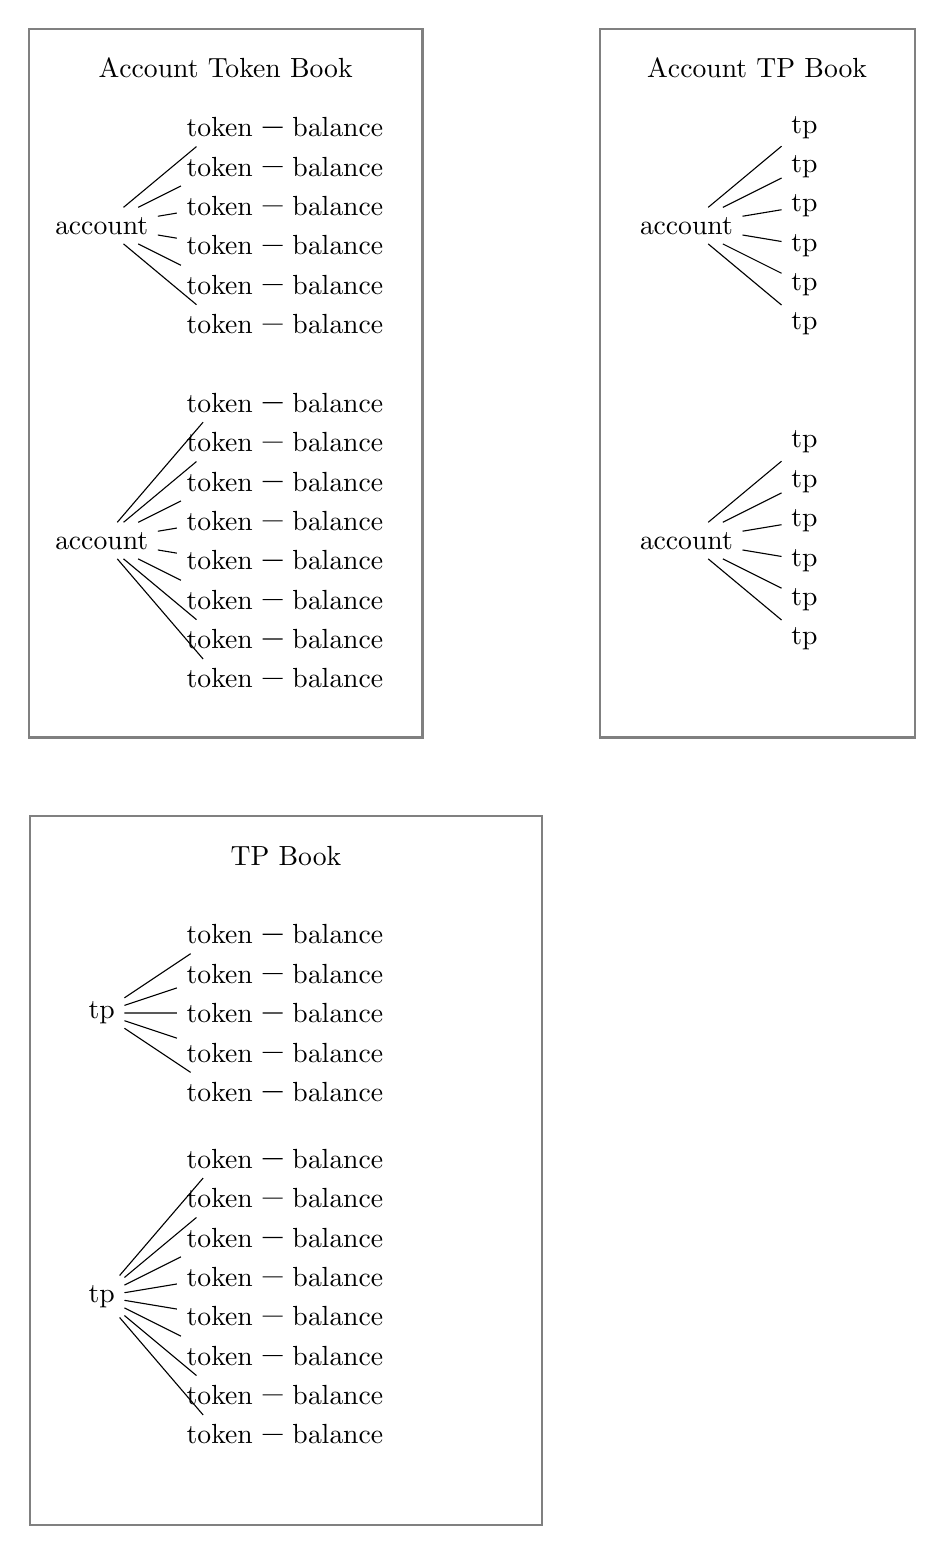
\begin{tikzpicture}[x=4.5cm,y=2cm]
        % Balance Book tree
        \node[style={draw,minimum width=5cm,minimum height=9cm,draw=black!50,thick}] (bbtreeoutline) at (0,0) {};
        \node[style={align=center,text width=4cm,text=black}] (bbtitle) at (0,2) {Account Token Book};
        \node (bbtree1) at (-.35,1) {account}[
                grow=east,
                level 1/.style = {sibling distance=.5cm}
            ]
            child {node {token} child {node {balance}} }
            child {node {token} child {node {balance}} }
            child {node {token} child {node {balance}} }
            child {node {token} child {node {balance}} }
            child {node {token} child {node {balance}} }
            child {node {token} child {node {balance}} };
        \node (bbtree2) at (-.35,-1) {account}[
                grow=east,
                level 1/.style = {sibling distance=.5cm}
            ]
            child {node {token} child {node {balance}} }
            child {node {token} child {node {balance}} }
            child {node {token} child {node {balance}} }
            child {node {token} child {node {balance}} }
            child {node {token} child {node {balance}} }
            child {node {token} child {node {balance}} }
            child {node {token} child {node {balance}} }
            child {node {token} child {node {balance}} };
        
        % Account TP Book tree
        \node[style={draw,minimum width=4cm,minimum height=9cm,draw=black!50,thick}] (tptreeoutline) at (1.5,0) {};
        \node[style={align=center,text width=4cm,text=black}] (tptitle) at (1.5,2) {Account TP Book};
        \node (tptree1) at (1.3,1) {account}[
                grow=east,
                level 1/.style = {sibling distance=.5cm},
                level 2/.style = {sibling distance=.5cm}
            ]
            child {node {tp}}
            child {node {tp}}
            child {node {tp}}
            child {node {tp}}
            child {node {tp}}
            child {node {tp}};
        \node (tptree2) at (1.3,-1) {account}[
                grow=east,
                level 1/.style = {sibling distance=.5cm},
                level 2/.style = {sibling distance=.5cm}
            ]
            child {node {tp}}
            child {node {tp}}
            child {node {tp}}
            child {node {tp}}
            child {node {tp}}
            child {node {tp}};

        % TP Book tree
        \node[style={draw,minimum width=6.5cm,minimum height=9cm,draw=black!50,thick}] (tptreeoutline) at (.17,-5) {};
        \node[style={align=center,text width=3cm,text=black}] (tptitle) at (.17,-3) {TP Book};
        \node (tptree1) at (-.35,-4) {tp}[
                grow=east,
                level 1/.style = {sibling distance=.5cm},
                level 2/.style = {sibling distance=.5cm}
            ]
            child {node {token} child {node {balance}} }
            child {node {token} child {node {balance}} }
            child {node {token} child {node {balance}} }
            child {node {token} child {node {balance}} }
            child {node {token} child {node {balance}} };
        \node (tptree2) at (-.35,-5.8) {tp}[
                grow=east,
                level 1/.style = {sibling distance=.5cm},
                level 2/.style = {sibling distance=.5cm}
            ]
            child {node {token} child {node {balance}} }
            child {node {token} child {node {balance}} }
            child {node {token} child {node {balance}} }
            child {node {token} child {node {balance}} }
            child {node {token} child {node {balance}} }
            child {node {token} child {node {balance}} }
            child {node {token} child {node {balance}} }
            child {node {token} child {node {balance}} };
        
    \end{tikzpicture}
\end{document}